\section{Task Formulation}
In this section, we formulate the task of automated hallucination judgment and attribution. 

\begin{figure*}[!t]
  \centering
    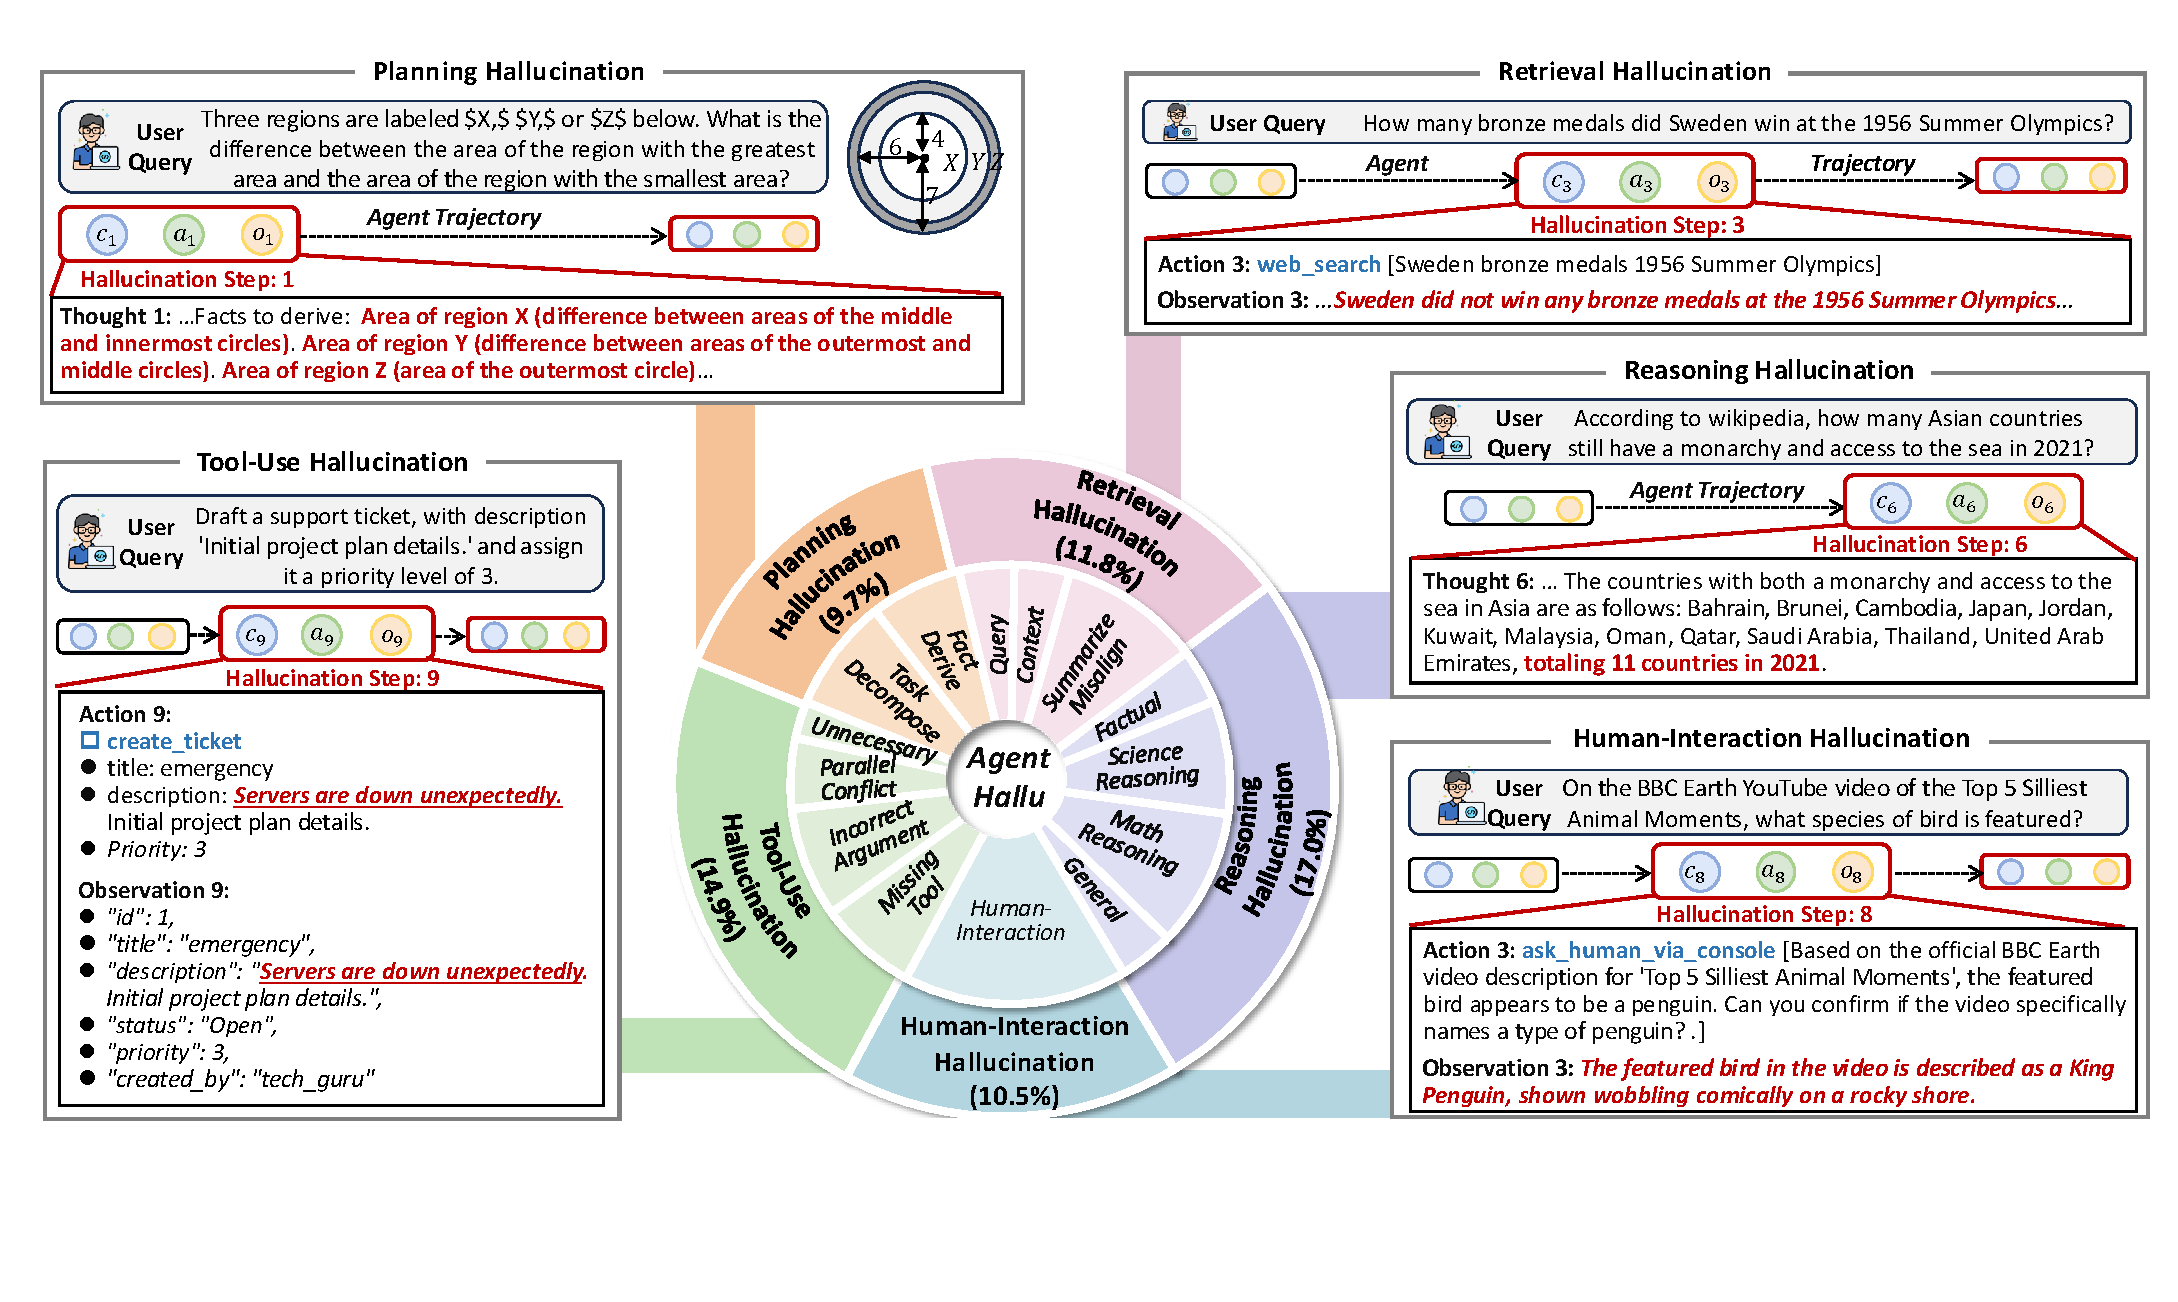
\includegraphics[width=1.0\linewidth]{Fig/dataset_illustration.pdf}
    % \vspace{-2.0em}
    \caption{ Overview of hallucination taxonomy in AgentHallu. The dataset includes 5 hallucination categories and 14 subcategories, where each trajectory step interleaves a thought step, an action step, and an observation step.
    }
    \label{fig:dataset_ills}
\end{figure*}

\paragraph{Background.} 
LLM-based agents perform complex tasks with structured reasoning, where each interaction unit $u_t$ interleaves a thought step $c_t$, an action step $a_t$, and an observation step $o_t$. The trajectory $\tau$ can be written as:
\begin{equation}
    \tau = (u_1, u_2, \ldots, u_t),
\end{equation}
\begin{equation}
    u_t = (c_t, a_t, o_t),
\end{equation}
where $c_t$ denotes the internal reasoning state, $a_t$ specifies the invoked tool action, and $o_t$ captures feedback from the tool responses.
Distinct from prior analyses of non-hallucination failures~\cite{zhang2025agent,cemri2025multi,rahardja2025can}, we restrict our study to trajectories that yield coherent and seemingly plausible answers.

\paragraph{Hallucination Judgment Objective.}
We classify a trajectory as hallucinated by determining whether its produced answer diverges from the ground-truth solution corresponding to the task:
\begin{equation}
    \mathrm{is\_hallucination}(\tau) = \mathbbm{1}_{\left\{ y(\tau) \neq y^{\mathrm{gt}} \right\}},
\end{equation}
where $y(\tau)$ denotes the result of a trajectory $\tau$, $y^{\mathrm{gt}}$ denotes the task-specific ground-truth answer, and $\mathbbm{1}_{\left\{ \cdot \right\}}$ is the indicator function.

\paragraph{Hallucination Attribution Objective.}
Motivated by~\cite{zhang2025agent}, we identify a hallucinated step $u_{t}$ as the step whose correction is causally sufficient to transform an incorrect result into a correct one. Specifically, we replace $u_{t}$ with its correct counterpart and roll out the subsequent steps to obtain the counterfactual trajectory $\tau^{(t)}$. The set of hallucinated steps $\mathcal{H}(\tau)$ of a trajectory $\tau$ is then defined as:
\begin{equation}
    \mathcal{H}(\tau) = \{\, t \mid y(\tau) \neq y^{\mathrm{gt}} \land y(\tau^{(t)}) = y^{\mathrm{gt}} \,\}, 
\end{equation}
where $y(\tau^{(t)})$ denotes the result produced by the counterfactual trajectory $\tau^{(t)}$.
To address scenarios with multiple hallucinated steps, we follow a \textbf{causality-aligned principle} and treat the initial error as the primary source of hallucination. We thus define an objective to determine:
\begin{equation}
    t^{\star}= \arg\min_{\, t \in \mathcal{H}(\tau)} \; t .
\end{equation}
In this study, we address the problem of automatically identifying the step $t^{\star}$ and providing an associated open-ended explanation.

\section{AgentHallu Dataset}
\label{sec:dataset}
In this section, we first present an overview of our AgentHallu dataset in Sec.~\ref{overview}. Then, we detail the dataset development involving query collection in Sec.~\ref{query_collection}, trajectory construction in Sec.~\ref{trajectory_construction}, and hallucination annotation in Sec.~\ref{hallucination_annotation}.

\subsection{Overview}
\label{overview}
As shown in Table~\ref{dataset_comparison} and Figure~\ref{fig:dataset_ills}, AgentHallu comprises 693 annotated agent trajectories, including 443 hallucinated instances and 250 non-hallucinated instances. Each instance in AgentHallu includes the following entries: \textbf{(1) Query:} A real-world question from 8 datasets, covering domains spanning world knowledge, science, math, general assistant, and tool use. \textbf{(2) Trajectory:} A trajectory generated to address the query, with each step standardized into a triplet of thought, action, and observation. These trajectories are collected from 7 mainstream LLM-based agents. \textbf{(3) Annotation:} Multi-level annotations curated by human labelers, comprising a binary label, a hallucination-responsible step, and a causal explanation. Detailed dataset statistics are provided in Appendix~\ref{appendix_data_statis}.

\subsection{Query Collection}
\label{query_collection}
To ensure comprehensive coverage of factuality, we curate a diverse set of queries spanning five realistic domains, as detailed below.
\begin{itemize}[noitemsep,left=2pt, itemsep=0pt, topsep=0pt]
    \item \textit{World Knowledge}: We incorporate queries from the SimpleQA dataset~\cite{wei2024measuring}, spanning ten topics such as politics, art, and sports to represent general world knowledge.
    \item \textit{Science}: We include graduate-level scientific queries from the GPQA dataset~\cite{rein2024gpqa}, involving the disciplines of physics, chemistry, and biology.
    \item \textit{Math}: We filter out difficulty Level 1 and Level 2 questions from MATH-500~\cite{hendrycks2021measuring}, retaining the harder subset. To integrate frontier-level challenges, we also include questions from the American Invitational Mathematics Examination (AIME) 2024 and AIME 2025.
    \item \textit{General Assistant}: We include queries from the GAIA validation set~\cite{mialon2023gaia}, which provides diverse and realistic instructions reflecting general assistant use.
    \item \textit{Tool Use}: To mimic complex tool-use sequences in agentic workflows, we incorporate multi-turn and multi-step function-calling queries from BFCL V3~\cite{patilberkeley}.
\end{itemize}
To extend coverage toward cutting-edge human knowledge, we also include a small subset of questions from HLE~\cite{phan2025humanity}, spanning mathematics, humanities, and the natural sciences.

\subsection{Trajectory Construction}
\label{trajectory_construction}
Given the collected queries, we generate diverse and realistic trajectories by executing 7 widely used LLM-based agents (SmolAgents~\cite{roucher2025smolagents}, OpenDeepSearch~\cite{alzubi2025open}, OpenManus~\cite{openmanus2025}, OctoTools~\cite{lu2025octotools}, Magentic-One~\cite{fourney2024magentic}, OWL~\cite{hu2025owl}, and Function-calling Agents~\cite{patilberkeley}). Specifically, we partition queries from the four knowledge-intensive domains into six subsets and instantiate trajectories using the first six agents. In parallel, we utilize BFCL V3 to construct function-calling agent trajectories. These agents are primarily built on the GPT series (GPT-4o and GPT-4.1). Details on agent configuration are provided in Appendix~\ref{appendix_agent_descrip}. 

To enhance the robustness and quality of our benchmark, we apply a three-stage filtering criterion to the collected trajectories: 
\begin{itemize}[noitemsep,left=2pt, itemsep=0pt, topsep=0pt]
    \item \textit{(1) Exclude Failure Trajectories}: Since non-deceptive failures are easy to identify, we manually exclude trajectories that terminate without a task-completing response (e.g., early termination due to turn limits, token overflows, or tool-permission restrictions).
    \item \textit{(2) Exclude Short Trajectories}: Excessively short agent trajectories degrade into native LLM responses, lacking sufficient reasoning depth for step localization. Therefore, we exclude trajectories with only one or two valid steps.
    \item \textit{(3) Exclude Trivial Trajectories}: To select plausible and difficult samples, we retain trajectories with disagreement among LLM judges. Specifically, we use four independent LLMs (\texttt{GPT-5}, \texttt{Gemini-2.5-Pro}, \texttt{DeepSeek-V3.1}, and \texttt{Qwen3-32B}) to assign a binary label and a hallucination-responsible step for each trajectory. Then we exclude trajectories with full agreement across all four judges.
\end{itemize}

\subsection{Hallucination Annotation}
\label{hallucination_annotation}
Through the multi-step filtering described above, we retain 693 agent trajectories. To ensure consistent and reproducible annotations across heterogeneous agent systems, we establish both an empirically grounded hallucination taxonomy and a standardized annotation protocol.

\begin{table}[t!]
    \centering
    \caption{Taxonomy of agent hallucinations.}
       \vspace{-0.5em}
    \label{category_description}
    \resizebox{\linewidth}{!}{
    \tablestyle{3.0pt}{1.3}
    \begin{tabular}{ll|l}
\hline
\rowcolor{COLOR_MEAN}
\textbf{Category}                                                                            & \textbf{Sub-category} & \textbf{Description}                            \\ \hline \hline
\multirow{2}{*}{\textbf{\begin{tabular}[c]{@{}l@{}}Planning \\ Hallucination\end{tabular}}}  & Fact Derive           & Introduce nonexistent or misleading facts.      \\
                                                                                             & Task Decompose        & Produce task-misaligned subgoals.               \\ \hline
\multirow{3}{*}{\textbf{\begin{tabular}[c]{@{}l@{}}Retrieval \\ Hallucination\end{tabular}}} & Query Misalign        & Formulate inaccurate retrieval queries.         \\
                                                                                             & Context Misalign      & Retrieve factually incorrect context.           \\
                                                                                             & Summarize Misalign    & Misrepresent context via summarization.         \\ \hline
\multirow{4}{*}{\textbf{\begin{tabular}[c]{@{}l@{}}Reasoning\\ Hallucination\end{tabular}}}  & Factual Reasoning     & Incorrect factual inference over context.       \\
                                                                                             & Math Reasoning        & Incorrect math inference or computation.        \\
                                                                                             & Science Reasoning     & Incorrect science inference or computation.     \\
                                                                                             & General Reasoning     & Incorrect reasoning over general tasks.         \\ \hline
\multicolumn{2}{l|}{\textbf{Human-Interaction Hallucination}}                                                        & Incorrect messages propagated by the user.      \\ \hline
\multirow{4}{*}{\textbf{\begin{tabular}[c]{@{}l@{}}Tool-Use \\ Hallucination\end{tabular}}}  & Missing Tool          & Miss required tool invocation.                  \\
                                                                                             & Incorrect Argument    & Mis-specify arguments of invoked tools.         \\
                                                                                             & Parallel Conflict     & Trigger execution conflicts via parallel tools. \\
                                                                                             & Unnecessary Tool      & Invoke irrelevant or incorrect tools.           \\ \hline
\end{tabular}
    }
\end{table}

% A: We develop an empirical taxonomy using grounded theory~\cite{glaser2017discovery}, which allows hallucination modes to emerge from empirical data. Specifically, we first curate a pilot set of 140 trajectories sampled from 7 agent frameworks. Then we conduct iterative open coding on the trajectory data to label observed hallucinated behaviors. Throughout this phase, we apply constant comparative analysis to refine the boundaries between different hallucination types. By merging and linking relevant behaviors, we organize the open codes into a structured taxonomy of hallucination categories. The taxonomy is further refined through discuss and review until consensus is reached. The resulting taxonomy is presented in Table~\ref{category_description}.
\noindent\textbf{Empirically Grounded Taxonomy.}
To allow hallucination modes to emerge from empirical data, we apply grounded theory~\cite{glaser2017discovery} to analyze a pilot set of 140 trajectories sampled from seven agent frameworks. Specifically, we first perform open coding~\cite{khandkar2009open} on the trajectory data to label observed hallucinated behaviors. Then we apply constant comparative analysis to refine the boundaries between different hallucination types. By merging and linking relevant behaviors, we organize the open codes into a structured taxonomy of hallucination categories. The taxonomy is finally refined through discussion and review until consensus is reached. The resulting taxonomy is presented in Table~\ref{category_description}.

\begin{table}[t!]
    \centering
    \caption{Initial inter-annotator agreement on binary judgment (\textbf{Judgment}), categorization (\textbf{Category}), and hallucination-responsible step (\textbf{Step}). The results highlight the difficulty of manual hallucination attribution.}
       \vspace{-0.5em}
    \label{agreement}
    \resizebox{\linewidth}{!}{
    \tablestyle{3.0pt}{1.2}
    \begin{tabular}{l||ccccc|c}
\hline
\rowcolor{COLOR_MEAN}
Annotation   & World. & Science & Math & General & Tool & Overall \\ \hline \hline
Judgment   & 98.4        & 98.0         & 100.0      & 100.0         & 98.8      & 98.9        \\
Category & 83.2        & 74.3         & 81.2      & 74.4         & 92.2     & 81.9        \\
Step     & 80.4        & 72.5         & 76.5      & 69.2         & 85.4     & 77.9        \\ \hline
\end{tabular}
    }
\end{table}






\begin{table*}[!t]
  \centering
%   \scriptsize
  \caption{Performance (\%) of LLMs on AgentHallu under standard prompting, reporting hallucination judgment (F1/Recall/Acc) and hallucination attribution measured by step localization accuracy (Acc) and G-EVAL (GE).}
       \vspace{-0.8em}
  \label{model_comparision}
    \resizebox{1.0\linewidth}{!}{
    \tablestyle{5.0pt}{1.15}
   \begin{tabular}{lccccccccccccccc}
\toprule
\multicolumn{1}{l|}{\multirow{3}{*}{\textbf{Model Name}}} & \multicolumn{3}{c|}{\textbf{Judgment}}                             & \multicolumn{12}{c}{\textbf{Attribution}}                                                                                                                                                                      \\ \cline{2-16} 
\multicolumn{1}{l|}{}                                     & \multicolumn{3}{c|}{Overall}                                       & \multicolumn{2}{c}{Planning} & \multicolumn{2}{c}{Retrieval} & \multicolumn{2}{c}{Reasoning} & \multicolumn{2}{c}{Human}    & \multicolumn{2}{c|}{Tool-Use}                         & \multicolumn{2}{c}{Overall}  \\ \cline{2-16} 
\multicolumn{1}{l|}{}                                     & F1$\uparrow$            & Recall$\uparrow$        & \multicolumn{1}{c|}{Acc$\uparrow$}           & Acc           & GE           & Acc            & GE           & Acc            & GE           & Acc           & GE           & Acc           & \multicolumn{1}{c|}{GE}           & Acc$\uparrow$           & GE$\uparrow$           \\ \midrule \midrule
\multicolumn{1}{c|}{Random}                               & 48.5          & 49.6          & \multicolumn{1}{c|}{49.5}          & 9.6           & -            & 8.8            & -            & 10.3           & -            & 7.4           & -            & 7.2           & \multicolumn{1}{c|}{-}            & 8.7           & -            \\ \midrule \midrule
\rowcolor{COLOR_MEAN}
\multicolumn{16}{l}{Proprietary Large Language Models}                                                                                                                                                                                                                                                                                          \\
\multicolumn{1}{l|}{GPT-5}                                &  \cellcolor{LightCyan}\textbf{70.2} & \cellcolor{LightCyan}\textbf{73.2} & \multicolumn{1}{c|}{\cellcolor{LightCyan}\textbf{70.6}} & \cellcolor{LightCyan}\textbf{31.3} & \cellcolor{LightCyan}\textbf{2.3} & 26.8           & 1.7          & 57.6           & 3.0          & 39.7          & 2.6          & 4.9           & \multicolumn{1}{c|}{0.6}          & 32.7          & 2.0          \\
\multicolumn{1}{l|}{GPT-5-mini}                           & 65.0          & 67.3          & \multicolumn{1}{c|}{65.5}          & 29.9          & 2.1          & 28.1           & 1.5          & 53.4           & 2.8          & \cellcolor{LightCyan}\textbf{61.6} & \cellcolor{LightCyan}\textbf{3.3} & 3.9           & \multicolumn{1}{c|}{0.6}          & 35.0          & 2.0          \\
\multicolumn{1}{l|}{Gemini-2.5-Pro}                       & 64.6          & 64.2          & \multicolumn{1}{c|}{68.8}          & 25.4          & 2.2          & \cellcolor{LightCyan}\textbf{45.1}  & \cellcolor{LightCyan}\textbf{2.3} & \cellcolor{LightCyan}\textbf{64.4}  & \cellcolor{LightCyan}\textbf{3.2} & 50.7          & 2.8          & 14.6          & \multicolumn{1}{c|}{1.3}          & \cellcolor{LightCyan}\textbf{41.1} & \cellcolor{LightCyan}\textbf{2.4} \\
\multicolumn{1}{l|}{Gemini-2.5-Flash}                     & 65.3          & 65.4          & \multicolumn{1}{c|}{67.7}          & 20.9          & 2.1          & 42.7           & 2.1          & 54.2           & 2.7          & 43.8          & 2.6          & 15.5          & \multicolumn{1}{c|}{1.3}          & 36.3          & 2.1          \\
\multicolumn{1}{l|}{Claude-4.5-Sonnet}                    & 63.6          & 63.7          & \multicolumn{1}{c|}{66.1}          & 26.9          & \cellcolor{LightCyan}\textbf{2.3}          & 30.5           & 1.7          & 44.9           & 2.3          & 43.8          & 2.4          & \cellcolor{LightCyan}\textbf{19.4} & \multicolumn{1}{c|}{\cellcolor{LightCyan}\textbf{1.4}} & 33.4          & 2.0          \\ \midrule
\multicolumn{1}{l|}{Average}                              & 65.7          & 66.8          & \multicolumn{1}{c|}{67.7}          & 26.9          & 2.2          & 34.6           & 1.9          & 54.9           & 2.8          & 47.9          & 2.7          & 11.6          & \multicolumn{1}{c|}{1.0}          & 35.7          & 2.1          \\ \midrule \midrule
\rowcolor{COLOR_MEAN}
\multicolumn{16}{l}{Open-source Large Language Models}                                                                                                                                                                                                                                                                                          \\
\multicolumn{1}{l|}{DeepSeek-V3.1}                        & \cellcolor{LightCyan}\textbf{52.1} & 52.1          & \multicolumn{1}{c|}{\cellcolor{LightCyan}\textbf{55.4}} & \cellcolor{LightCyan}\textbf{14.9} & \cellcolor{LightCyan}\textbf{1.8} & 22.0           & \cellcolor{LightCyan}\textbf{1.6} & 27.1           & \cellcolor{LightCyan}\textbf{1.8} & 21.9          & 1.9          & 7.8           & \multicolumn{1}{c|}{\cellcolor{LightCyan}\textbf{0.7}} & 19.0          & \cellcolor{LightCyan}\textbf{1.5} \\
\multicolumn{1}{l|}{Qwen3-32B}                            & 51.8          & 53.0          & \multicolumn{1}{c|}{52.7}          & 7.5           & 1.5          & 19.5           & 1.1          & \cellcolor{LightCyan}\textbf{28.8}  & 1.7          & \cellcolor{LightCyan}\textbf{41.1} & \cellcolor{LightCyan}\textbf{2.1} & \cellcolor{LightCyan}\textbf{8.7}  & \multicolumn{1}{c|}{0.5}          & \cellcolor{LightCyan}\textbf{21.2} & 1.3          \\
\multicolumn{1}{l|}{Qwen3-8B}                             & 49.5          & 54.2          & \multicolumn{1}{c|}{49.5}          & 4.5           & 1.2          & \cellcolor{LightCyan}\textbf{28.1}  & 1.3          & 17.0           & 0.9          & 23.3          & 1.2          & 3.9           & \multicolumn{1}{c|}{0.2}          & 15.1          & 0.9          \\
\multicolumn{1}{l|}{Qwen2.5-72B}                          & 44.3          & 55.2          & \multicolumn{1}{c|}{46.0}          & 4.5           & 0.8          & 3.7            & 0.3          & 9.3            & 0.6          & 13.7          & 0.7          & 6.8           & \multicolumn{1}{c|}{0.5}          & 7.7           & 0.6          \\
\multicolumn{1}{l|}{Qwen2.5-32B}                          & 49.3          & \cellcolor{LightCyan}\textbf{56.3} & \multicolumn{1}{c|}{49.6}          & 4.5           & 1.1          & 1.2            & 0.5          & 15.3           & 0.9          & 12.3          & 0.8          & 6.8           & \multicolumn{1}{c|}{0.6}          & 8.6           & 0.8          \\
\multicolumn{1}{l|}{Qwen2.5-7B}                           & 43.9          & 51.1          & \multicolumn{1}{c|}{44.2}          & 0.0           & 0.6          & 6.1            & 0.5          & 5.9            & 0.4          & 13.7          & 0.8          & 6.8           & \multicolumn{1}{c|}{0.5} & 6.6           & 0.5          \\
\multicolumn{1}{l|}{Llama3.3-70B}                         & 40.4          & 54.2          & \multicolumn{1}{c|}{43.6}          & 10.5          & 0.9          & 4.9            & 0.4          & 6.8            & 0.3          & 5.5           & 0.3          & \cellcolor{LightCyan}\textbf{8.7}  & \multicolumn{1}{c|}{0.5}          & 7.2           & 0.4          \\
\multicolumn{1}{l|}{Llama3.1-8B}                          & 35.1          & 52.1          & \multicolumn{1}{c|}{40.3}          & 0.0           & 0.3          & 2.4            & 0.3          & 0.9            & 0.2          & 4.1           & 0.2          & 1.0           & \multicolumn{1}{c|}{0.1}          & 1.6           & 0.2          \\ \midrule
\multicolumn{1}{l|}{Average}                              & 45.8          & 53.5          & \multicolumn{1}{c|}{47.7}          & 5.8           & 1.0          & 11.0           & 0.8          & 13.9           & 0.8          & 17.0          & 1.0          & 6.3           & \multicolumn{1}{c|}{0.4}          & 10.9          & 0.8          \\ \bottomrule
\end{tabular}
}
\end{table*}






\noindent\textbf{Standardized Annotation Protocol.}
We introduce a hallucination annotation protocol, which progresses from binary judgment to fine-grained attribution and taxonomy classification. To ensure annotation rigor, we employ ten graduate-level annotators with specialized expertise in AI to perform iterative labeling and refinement.
\begin{itemize}[noitemsep,left=2pt, itemsep=0pt, topsep=0pt]
    \item \textit{(1) Construction of Oracle-guided Reasoning Paths}. Considering that hallucination attribution often requires domain-specific expertise, we leverage LLMs to 
    construct detailed reasoning paths for question solving. Specifically, we condition the LLM on the question, the ground-truth answer, and, when available, dataset-provided solution annotations. Compared with question-only prompting, providing this additional information yields more faithful reasoning paths. To mitigate model-specific bias, each path is independently drafted by two different LLMs, GPT-5-Thinking and Gemini-2.5-Pro.   
    \item \textit{(2) Human Annotation}. Annotators first make a binary judgment of whether the agent trajectory is hallucinated by comparing it with the ground truth. For hallucinated cases, they further annotate the category, hallucination-responsible step, and causal explanation. To facilitate this process, LLMs are prompted with the reasoning path to generate attribution references, which are subsequently verified by annotators. Validation relies on two criteria: whether the candidate step introduces a factual error that directly distorts the outcome, or whether it propagates an error seeded in an earlier step. Upon detecting such propagation, annotators trace the error chain backward and reassign attribution to the root cause.
    \item \textit{(3) Consensus Resolution}. Inter-annotator agreement statistics are reported in Table~\ref{agreement}. For disagreements, annotations are resolved through collaborative discussion, requiring all annotators to be convinced by the final rationale. For agreed cases, we employ a cross-validation protocol in which each annotator reviews peer annotations to ensure adherence to shared standards. Any detected inconsistency triggers discussion and re-annotation until consensus is achieved.    
\end{itemize}





